\chapter{Moleculaire plantenfysiologie en stressreacties}\label{ch:b3:plant-molecular-physiology}

Een boneplantje dat in een donkere kast is opgekweekt is een bleek,
spichtig ding: een lange witte stengel, een haak bovenaan, twee
gevouwen gele blaadjes. Zet het voor een raam en binnen een dag is het
opgehouden met strekken, heeft het zijn haak gestrekt en zijn blaadjes
uitgespreid en groen gemaakt --- een ander organisme, uit dezelfde
genen. Het had niet op energie gewacht; het had op informatie gewacht.
Eén rood foton dat door één eiwit wordt opgenomen vertelt het dat het
het licht heeft bereikt; de verhouding van rood tot verrood vertelt het
of er een blad van een buur boven hangt; de lengte van de nacht vertelt
het het jaargetijde; een daling van de waterpotentiaal van zijn
wortels, een vleug wind, het flagelline van een bacterie op zijn blad
--- elk wordt door een receptor waargenomen, omgezet in een chemisch
signaal en beantwoord met een verandering in welke genen tot expressie
komen en welke cellen groeien. Een plant kan niet voor haar omgeving
weglopen; zij moet die lezen en zichzelf verbouwen. Dit hoofdstuk gaat
over dat lezen: de fotoreceptoren, de \omterm{def:b3:endocrinology:hormone}{hormonen} en hoe zij op
moleculaire schaal werken, de reacties op droogte, zout, koude en
hitte, en het afweersysteem met twee lagen dat planten hebben
ontwikkeld zonder ook maar één beweeglijke cel.

\section{Het licht lezen}

\begin{definition}[Fotoreceptoren]\label{def:b3:plant-molecular-physiology:photoreceptors}
\index{fytochroom}\index{cryptochroom}\index{fototropine}\index{fotomorfogenese}\index{etiolering}
Planten nemen licht waar met drie eiwitfamilies, waarvan geen enkele
chlorofyl is. \emph{Fytochromen} zijn dimeren met een bilinepigment dat
door rood licht (\qty{660}{nm}) van de inactieve \emph{Pr}-vorm naar de
actieve \emph{Pfr} wordt omgezet, en door verrood (\qty{730}{nm}) weer
terug; Pfr gaat de kern in en merkt een familie transcriptiefactoren,
de PIF's, voor afbraak, waarmee het de genen van de ontwikkeling in het
licht vrijgeeft; in het donker keert Pfr langzaam terug.
\emph{Cryptochromen} (blauw, \qty{450}{nm}) zijn flavo-eiwitten die
verwant zijn aan enzymen voor DNA-herstel en die de de-etiolering, de
klok en de bloei besturen; \emph{fototropinen} (blauw) zijn
membraankinasen die het buigen naar het licht, het openen van de
huidmondjes en de beweging van de chloroplasten sturen. Een kiemplant
in het donker is \emph{geëtioleerd} --- een lang hypocotyl, gesloten
zaadlobben, geen chlorofyl, alle middelen besteed aan het bereiken van
het oppervlak; licht schakelt haar om naar de \emph{fotomorfogenese},
en die schakelaar wordt omgezet doordat Pfr en cryptochroom één enkel
repressorcomplex (COP1) uitschakelen dat in het donker de
transcriptiefactoren van het lichtprogramma vernietigt. Licht wordt dus
tweemaal gelezen: als energie, door de chloroplast, en als signaal,
door receptoren die gevoelig zijn voor fotonenstromen die een miljoen
maal kleiner zijn.
\end{definition}

\begin{proposition}[Het foto-evenwicht van fytochroom]\label{prop:b3:plant-molecular-physiology:photoequilibrium}
\index{foto-evenwicht}\index{rood-verroodverhouding}\index{schaduwontwijking}
Onder aanhoudend licht gaan Pr en Pfr in elkaar over tot de twee
omzettingssnelheden in evenwicht zijn: met $k_{1}$ de snelheid van Pr $\to$ Pfr
(evenredig met de rode stroom) en $k_{2}$ die van Pfr $\to$ Pr
(evenredig met de verrode stroom, plus een weinig uit het rood, dat Pfr
ook opneemt), is het deel in de actieve vorm
\[
\varphi = \frac{[\text{Pfr}]}{[\text{Pfr}] + [\text{Pr}]} = \frac{k_{1}}{k_{1} + k_{2}},
\]
onafhankelijk van de totale stroom en alleen bepaald door de
\emph{rood-verroodverhouding} $\zeta$ van het licht. Zuiver rood geeft
$\varphi \approx 0.87$ (Pfr neemt ook wat rood op), zuiver verrood
$0.03$; open daglicht, $\zeta \approx
1.15$, geeft ongeveer $0.55$, en het licht onder een bladerdak, wier
chlorofyl het rood eruit heeft gehaald en het verrood heeft
doorgelaten, heeft $\zeta \approx 0.2$ en $\varphi \approx 0.2$. Een
plant leest haar $\varphi$ als de aanwezigheid van buren: een lage
waarde lokt het syndroom van de \emph{\omterm{prop:b3:plant-molecular-physiology:photoequilibrium}{schaduwontwijking}} uit ---
gestrekte stengels, opgerichte bladeren, vroege bloei, minder
vertakking --- via de PIF's die Pfr niet meer vernietigt. De dichte
aanplant van een boer is een wedloop van schaduwontwijkers; de
dwergtarwes van de groene revolutie, ongevoelig voor het signaal,
staken de bespaarde groei in het graan.
\end{proposition}
\begin{proof}
$\mathrm{d}[\text{Pfr}]/\mathrm{d}t = k_{1}[\text{Pr}] - k_{2}[\text{Pfr}]$
met een vaste $[\text{Pr}] + [\text{Pfr}] = P$ geeft in de stationaire
toestand $k_{1}(P - [\text{Pfr}]) = k_{2}[\text{Pfr}]$, waaruit $\varphi = k_{1}/
(k_{1} + k_{2})$. Beide snelheden zijn evenredig met de invallende
stroom, dus schalen zij beide mee wanneer het licht wordt geschaald en
blijft $\varphi$ onveranderd; alleen de spectrale samenstelling telt.
De stationaire toestand wordt genaderd met snelheid $k_{1} + k_{2}$ ---
seconden in zonlicht, minuten in de schemering --- en de terugkeer van
Pfr in het donker, met een halveringstijd van uren, bepaalt wat er
's nachts overblijft.
\end{proof}

\begin{omfigure}
\begin{tikzpicture}[every node/.style={font=\scriptsize}, >=stealth]
  \node[draw, very thick, omDef, fill=omDef!15, rounded corners, minimum width=1.6cm, minimum height=0.9cm] (pr) at (0,0) {Pr (inactief)};
  \node[draw, very thick, omThm, fill=omThm!15, rounded corners, minimum width=1.6cm, minimum height=0.9cm] (pfr) at (4.2,0) {Pfr (actief)};
  \draw[->, very thick, red!70!black] (pr.north east) to[bend left=25] node[above] {rood, \qty{660}{nm}} (pfr.north west);
  \draw[->, very thick, red!40!black] (pfr.south west) to[bend left=25] node[below] {verrood, \qty{730}{nm}} (pr.south east);
  \draw[->, thick, gray] (pfr.south) ++(0.5,-0.15) to[bend left=40] node[right, font=\tiny, gray] {terugkeer in het donker, uren} ++(-0.3,-0.9);
  \draw[->, thick] (pfr.east) -- ++(1.0,0) node[right, align=left] {de kern in:\\PIF's afgebroken, COP1 uit;\\lichtprogramma aan};
  \begin{scope}[shift={(0,-4.6)}]
  \begin{axis}[
    width=0.55\linewidth, height=4.6cm,
    axis x line=bottom, axis y line=left,
    xmin=0, xmax=2.5, ymin=0, ymax=1,
    xlabel={rood-verroodverhouding $\zeta$}, ylabel={$\varphi = $ Pfr-fractie},
    xlabel style={font=\scriptsize, at={(axis description cs:0.5,-0.15)}, anchor=north}, ylabel style={font=\scriptsize},
    tick label style={font=\scriptsize}, xtick={0.2,0.5,1.15,2}, xticklabels={0.2,0.5,1.15,2}, ytick={0.2,0.55,0.87},
    clip=false,
  ]
  \addplot[very thick, omDef, domain=0:2.5, samples=80] {0.87*x/(x+0.6)};
  \draw[dashed, gray] (axis cs:0.2,0) -- (axis cs:0.2,0.22) -- (axis cs:0,0.22);
  \draw[dashed, gray] (axis cs:1.15,0) -- (axis cs:1.15,0.57) -- (axis cs:0,0.57);
  \node[font=\tiny, anchor=west, align=left] at (axis cs:0.25,0.12) {onder een bladerdak:\\schaduwontwijking};
  \node[font=\tiny, anchor=south west] at (axis cs:1.2,0.62) {open daglicht};
  \node[font=\tiny, anchor=north west, omDef, align=left] at (axis cs:1.6,0.45) {een empirische fit,\\$\varphi \approx 0.87\,\zeta/(\zeta + 0.6)$};
  \end{axis}
  \end{scope}
\end{tikzpicture}

{\small De schakelaar van het \omterm{def:b3:plant-molecular-physiology:photoreceptors}{fytochroom}. Rood licht maakt de actieve
vorm, verrood maakt haar ongedaan, het donker laat haar langzaam
terugkeren; het blijvende deel in de actieve vorm hangt af van de
kleurbalans van het licht en niet van de helderheid, en zo weet een
kiemplant dat er een blad boven haar hangt.}
\end{omfigure}

\begin{proof}[Bewijsmateriaal]
Borthwick, Hendricks en collega's (1952) gaven zaden van sla korte
flitsen: rood liet ze ontkiemen, verrood daarna gegeven maakte dat
ongedaan, opnieuw rood herstelde het, en zo voort door een dozijn
afwisselingen --- de laatste flits besliste, het kenmerk van een
omkeerbaar pigment, dat zij daarna (1959) als een blauw eiwit
uittrokken dat zijn absorptiespectrum onder rood en verrood veranderde.
Later bleek het hele programma van de in het donker gegroeide kiemplant
aan één repressor te hangen: mutanten zonder COP1 ontwikkelen zich in
volslagen duisternis als in het licht, kort en klaar om te vergroenen,
en mutanten zonder \omterm{def:b3:plant-molecular-physiology:photoreceptors}{fytochroom} of \omterm{def:b3:plant-molecular-physiology:photoreceptors}{cryptochroom} blijven in het licht
geëtioleerd.
\end{proof}

\begin{omfigure}
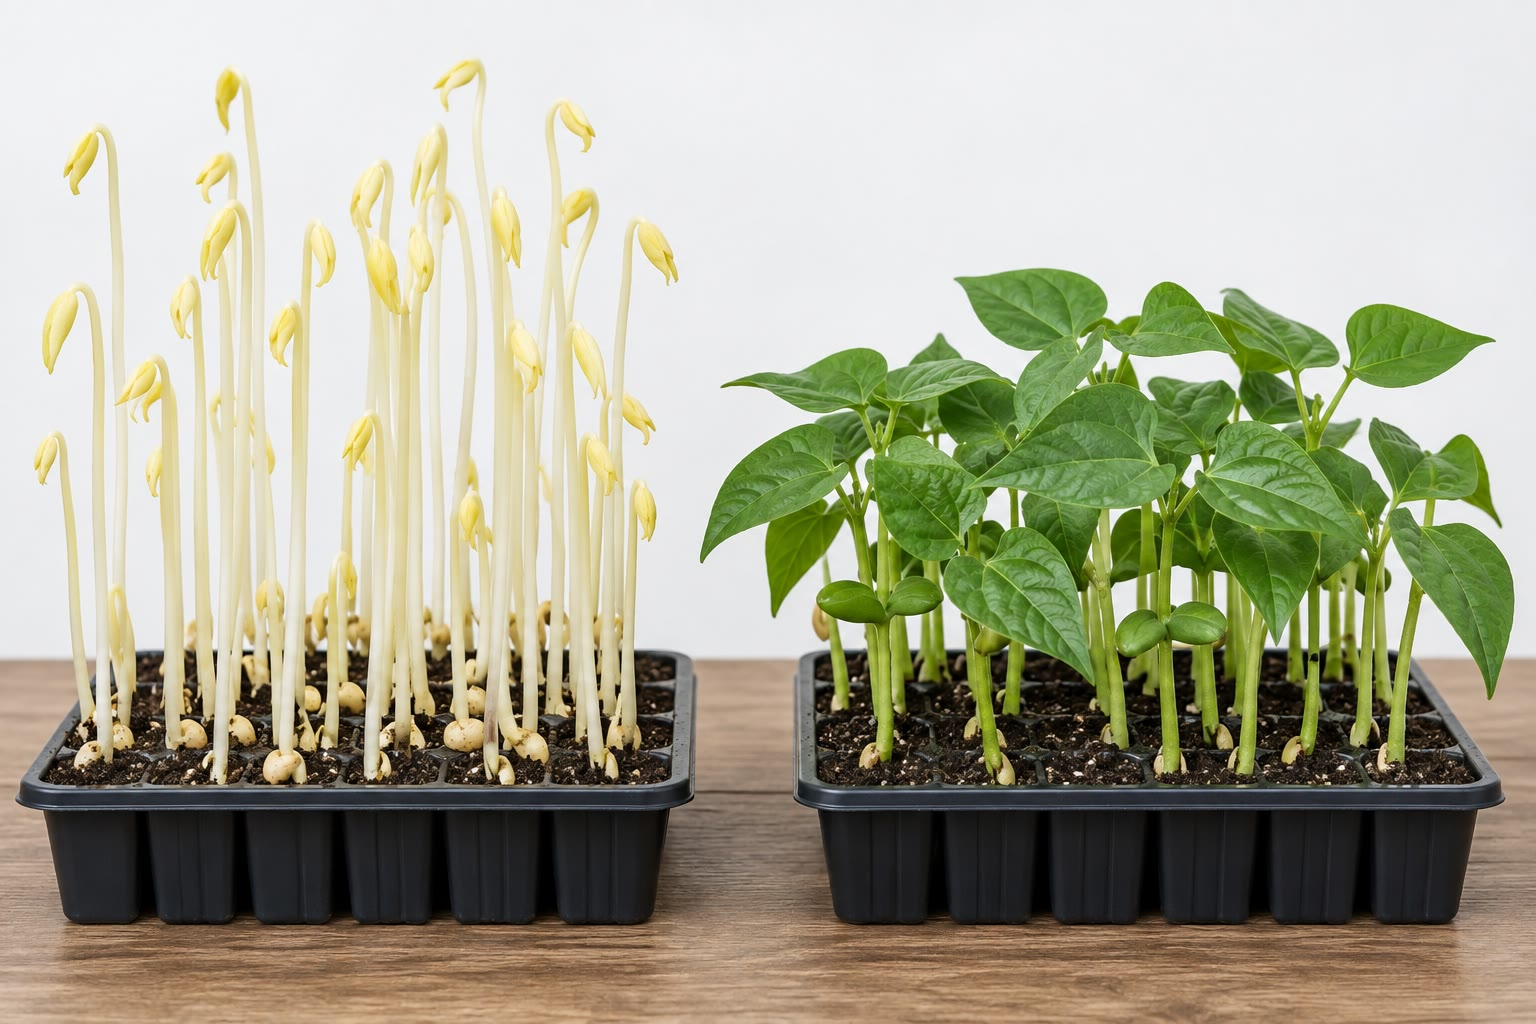
\includegraphics[width=0.56\linewidth]{images/book5/ai/b5-22-etiolated-seedlings.jpg}

{\small Kiemplanten opgekweekt in het donker en in het licht: hetzelfde
genoom, twee ontwikkelingsprogramma's, en het verschil is één rood
foton dat door \omterm{def:b3:plant-molecular-physiology:photoreceptors}{fytochroom} wordt opgenomen.}
\end{omfigure}

\section{Hormonen op moleculaire schaal}

\begin{definition}[De plantenhormonen en hun receptoren]\label{def:b3:plant-molecular-physiology:hormones}
\index{auxine}\index{TIR1}\index{gibberelline}\index{DELLA}\index{abscisinezuur}\index{ethyleen}\index{cytokinine}\index{brassinosteroïde}
Het deel van het eerste jaar beschreef wat de plantenhormonen doen;
hier staat hoe zij worden gehoord. Verscheidene werken door
\emph{geregelde vernietiging}. \emph{Auxine} (indool-3-azijnzuur) bindt
het F-box-eiwit \emph{TIR1} en lijmt het aan de Aux/IAA-repressoren,
die daarna door het proteasoom worden geubiquitineerd en vernietigd: de
genen van het auxine-antwoord die zij onderdrukten gaan binnen minuten
aan --- het \omterm{def:b3:endocrinology:hormone}{hormoon} is een moleculaire lijm, en de receptor maakt deel
uit van de afbraakmachinerie. \emph{Gibberelline} doet hetzelfde met de
\emph{DELLA}-repressoren van de groei, via zijn receptor GID1: de
dwergtarwes en dwergrijsten van de groene revolutie dragen
DELLA-eiwitten die niet kunnen worden vernietigd, en blijven dus kort
hoeveel gibberelline zij ook maken. \emph{Jasmonaat} volgt dezelfde
logica met de JAZ-repressoren. \emph{Abscisinezuur} (ABA), het \omterm{def:b3:endocrinology:hormone}{hormoon}
van droogte en kiemrust, bindt de PYR/PYL-receptoren, die daarna een
fosfatase (PP2C) remmen en zo een kinase (SnRK2) vrijmaken dat
ionkanalen en transcriptiefactoren fosforyleert --- een dubbele
ontkenning die het antwoord steil maakt. \emph{Ethyleen}, een gas,
bindt koperhoudende receptoren in het membraan van het ER die het
antwoord bij afwezigheid ervan actief onderdrukken; binding zet ze uit,
en de genen voor rijping, veroudering en stress gaan aan.
\emph{Cytokininen} werken via receptoren met een histidinekinase, als
de tweecomponentensystemen van bacteriën; \emph{brassinosteroïden}, de
steroïden van de plant, via een receptorkinase aan het oppervlak en
niet via een \omterm{def:b3:endocrinology:hormone}{kernreceptor} --- de enige steroïdhormonen waar ook ter
wereld die aan het celoppervlak worden gehoord. Planten hebben geen
klieren: elk \omterm{def:b3:endocrinology:hormone}{hormoon} wordt gemaakt waar het nodig is, of door eigen
transporteiwitten verplaatst, en zijn concentratie wordt plaatselijk
bepaald door aanmaak, conjugatie en vernietiging.
\end{definition}

\begin{theorem}[Chemiosmotisch polair transport van auxine]\label{thm:b3:plant-molecular-physiology:auxin}
\index{polair auxinetransport}\index{PIN-eiwitten}\index{anionenval}
Indool-3-azijnzuur is een zwak zuur, $\mathrm{p}K_{a} = 4.75$. In de
ruimte van de celwand bij pH~$5.5$ is een aanzienlijk deel het neutrale
IAAH, dat door het membraan diffundeert; in het cytosol bij pH~$7.2$ is
vrijwel alles het anion IAA$^{-}$, dat er niet door diffusie uit kan.
Bij evenwicht van de neutrale vorm over het membraan is de verhouding
van het totale \omterm{def:b3:plant-molecular-physiology:hormones}{auxine} binnen tot buiten
\[
\frac{[\text{IAA}]_{\text{in}}}{[\text{IAA}]_{\text{out}}}
= \frac{1 + 10^{\,\mathrm{pH}_{\text{in}} - \mathrm{p}K_{a}}}{1 + 10^{\,\mathrm{pH}_{\text{out}} - \mathrm{p}K_{a}}}
\approx \frac{283}{6.6} \approx 43 :
\]
vangt de cel het \omterm{def:b3:plant-molecular-physiology:hormones}{auxine} veertigvoudig. Het kan alleen naar buiten via
de \emph{PIN}-uitvoertransporteiwitten, en omdat elke cel haar PIN's op
één vlak zet --- het basale vlak in de stengel --- verlaat het \omterm{def:b3:plant-molecular-physiology:hormones}{auxine}
dat rondom is opgenomen de cel aan de onderkant, gaat de volgende cel
binnen, en zo voort: een kolom cellen met dezelfde polariteit is een
lopende band die \omterm{def:b3:plant-molecular-physiology:hormones}{auxine} met ongeveer \qty{1}{cm/h} van de scheuttop
naar de wortel verplaatst, en de PIN's anders richten stuurt de stroom
de andere kant op, en zo komt de beschaduwde kant van een stengel aan
meer \omterm{def:b3:plant-molecular-physiology:hormones}{auxine} en groeit zij sneller.
\end{theorem}
\begin{proof}
Henderson--Hasselbalch: $[\text{IAA}^{-}]/[\text{IAAH}] = 10^{\,\mathrm{pH}
- \mathrm{p}K_{a}}$, dus totaal $= [\text{IAAH}](1 + 10^{\,\mathrm{pH} -
\mathrm{p}K_{a}})$. De neutrale vorm komt in evenwicht, $[\text{IAAH}]_{\text{in}}
= [\text{IAAH}]_{\text{out}}$; de totalen op elkaar delen geeft de
verhouding, $(1 + 10^{2.45})/(1 + 10^{0.75}) = 283/6.6$. Met de PIN's
op één vlak is de enige uitgang van het anion gericht; een kolom van
$n$ cellen geeft de stroom door, en de gemeten snelheid, een orde van
grootte boven de diffusie over deze afstanden, is die van door
transporteiwitten verzorgde uitvoer bij elke celgrens. De hypothese van
Cholodny en Went (jaren 1920), dat het buigen een zijdelingse
herverdeling van \omterm{def:b3:plant-molecular-physiology:hormones}{auxine} volgt, werd bevestigd door rechtstreekse meting
in coleoptielen van haver en door het in beeld brengen van de
verplaatsing van PIN in wortels van \emph{Arabidopsis} die op hun zij
waren gelegd (jaren 2000).
\end{proof}

\begin{omfigure}
\begin{tikzpicture}[every node/.style={font=\scriptsize}, >=stealth]
  % three cells in a column
  \foreach \y in {0,-2.2,-4.4} {
    \draw[thick, omDef, fill=omDef!8] (0,\y) rectangle (3.2,\y-1.9);
    \draw[very thick, omThm] (0.6,\y-1.9) -- (2.6,\y-1.9);
    \node[right, font=\tiny] at (3.3,\y-0.4) {cytosol op pH 7.2};
    \node[right, font=\tiny] at (3.3,\y-0.8) {IAA$^{-}$ gevangen};
    \draw[->, thick, omDef!70!black] (-0.6,\y-0.6) -- (0.4,\y-0.6); \node[left, font=\tiny] at (-0.6,\y-0.6) {IAAH naar binnen};
    \draw[->, thick, omDef!70!black] (3.8,\y-1.3) -- (2.8,\y-1.3);
    \draw[->, very thick, omThm] (1.6,\y-1.5) -- (1.6,\y-2.35);
  }
  \node[left, align=right, font=\tiny] at (-0.6,-1.4) {celwand op pH 5.5:\\\qty{15}{\%} IAAH,\\\qty{85}{\%} IAA$^{-}$};
  \node[omThm, right, font=\tiny] at (3.3,-2.05) {PIN-uitvoereiwitten, alleen op het basale vlak};
  \node[above] at (1.6,0.1) {scheuttop: bron van auxine};
  \node[below] at (1.6,-6.8) {naar de wortel, \qty{1}{cm/h}};
  \node[right, align=left] at (5.4,-3.6) {binnen : buiten $\approx 43 : 1$\\(de anionenval)\\[3pt]uitgang alleen via PIN's,\\dus is de kolom een lopende band;\\verplaats de PIN's naar een zijvlak\\en de stroom draait};
\end{tikzpicture}

{\small Het chemiosmotische model van het \omterm{thm:b3:plant-molecular-physiology:auxin}{polaire auxinetransport}. Het
zuur komt langs elk vlak binnen als het neutrale molecuul, wordt bij de
pH van het cytosol als anion gevangen, en vertrekt alleen via
transporteiwitten die de cel op één vlak heeft gezet --- zodat een rij
cellen \omterm{def:b3:plant-molecular-physiology:hormones}{auxine} in één richting doorgeeft.}
\end{omfigure}

\begin{example}[Gravitropie en fototropie]\label{ex:b3:plant-molecular-physiology:tropism}
Leg een kiemplant op haar zij. In het wortelmutsje zakken dichte, met
zetmeel gevulde plastiden binnen minuten naar de nieuwe onderkant van
de columellacellen; de PIN3-transporteiwitten van die cellen verhuizen
naar het onderste vlak; \omterm{def:b3:plant-molecular-physiology:hormones}{auxine} stroomt bij voorkeur langs de onderste
flank van de wortel, waar het, boven het optimum voor wortelcellen, de
strekking \emph{remt}, en de wortel buigt omlaag. In de scheut
\emph{bevordert} dezelfde zijdelingse stroom naar de onderkant de
strekking (het optimum van scheutcellen ligt hoger), en de scheut buigt
omhoog. Fototropie: \omterm{def:b3:plant-molecular-physiology:photoreceptors}{fototropine} aan de belichte kant van een scheut
verandert de plaatsing van de PIN's zodat \omterm{def:b3:plant-molecular-physiology:hormones}{auxine} zich aan de
beschaduwde kant ophoopt, die sneller groeit en de scheut naar het
licht buigt. Beide bewegingen zijn traag --- uren --- omdat het groei
is en geen beweging, en beide zijn onomkeerbaar in het weefsel dat is
gegroeid. Darwin (1880) liet zien dat de top van een graskiemplant het
licht waarneemt en dat het gebied eronder buigt; Went (1928) ving de
invloed op in een agarblokje dat op een afgesneden top was gezet en
toonde dat een blokje dat scheef op een onthoofde scheut werd gezet die
deed buigen: de invloed was een diffundeerbare stof, die daarna \omterm{def:b3:plant-molecular-physiology:hormones}{auxine}
werd genoemd.
\end{example}

\section{Water, zout, koude en hitte}

\begin{definition}[Abiotische stress]\label{def:b3:plant-molecular-physiology:abiotic}
\index{droogtestress}\index{osmotische aanpassing}\index{zoutstress}\index{koude-acclimatisatie}\index{hitteschok-eiwitten}
Een plant kan niet ontsnappen, dus hardt zij zich. \emph{Droogte}: een
dalende waterpotentiaal in de wortels zet de aanmaak van ABA in gang;
ABA sluit de huidmondjes binnen minuten en zet in de loop van dagen de
genen aan voor \emph{osmotische aanpassing} (proline, suikers en andere
verenigbare opgeloste stoffen hopen zich op en verlagen de
waterpotentiaal van de cel, zodat zij water blijft aantrekken), voor
dehydrinen die eiwitten beschermen, en voor een kleiner bladoppervlak
en een diepere wortel. \emph{Zout} is droogte plus vergif: natrium komt
door kaliumkanalen binnen en wedijvert met kalium; verdraagzame planten
pompen het de wortels weer uit (de SOS-route), de vacuolen in
(NHX-uitwisselaars), of scheiden het uit via klieren op het blad, en
hun uiterste, de \emph{halofyt}, leeft in zeewater. \emph{Koude}: kilte
maakt membranen stijf en vertraagt enzymen; vriezen trekt water uit de
cellen naar ijs buiten de cel en droogt ze uit.
\emph{Koude-acclimatisatie} --- een week koele dagen --- wekt de
CBF-transcriptiefactoren op, die honderden genen aanzetten voor lipiden
die het membraan vloeiend houden, suikers, antivrieseiwitten en
dehydrinen, en een winterrogge die in augustus bij \qty{-5}{\celsius}
zou sterven overleeft in januari \qty{-30}{\celsius}. \emph{Hitte}
ontvouwt eiwitten; binnen minuten na een stijging maakt een
hitteschokfactor \emph{hitteschok-eiwitten} vrij, \omterm{def:b3:structural-biology:chaperones}{chaperonnes} die ze
weer opvouwen of opruimen, uit dezelfde families als in elk organisme.
\emph{Overstroming} berooft de wortels van zuurstof; rijst maakt
luchtkanalen (aerenchym) en strekt zich om haar bladeren boven water te
houden, waarbij \omterm{def:b3:plant-molecular-physiology:hormones}{ethyleen} het signaal is dat zich ophoopt wanneer het
niet in het water kan ontsnappen. Veel van deze programma's overlappen
--- ABA, reactieve zuurstofdeeltjes en calciumpieken zijn gedeelde
tweede boodschappers --- en een plant die aan de ene stress is gewend
is vaak ten dele tegen een andere beschermd.
\end{definition}

\begin{proposition}[Het huidmondje als klep]\label{prop:b3:plant-molecular-physiology:stomata}
\index{huidmondje}\index{sluitcel}\index{geleiding van het huidmondje}\index{watergebruiksefficiëntie}
Een paar \emph{\omterm{prop:b3:plant-molecular-physiology:stomata}{sluitcellen}} begrenst elke opening van een huidmondje;
de opening gaat open wanneer zij kalium en anionen opnemen (en suiker
maken), zwellen en uit elkaar buigen, en gaat dicht wanneer zij die
verliezen. Blauw licht (\omterm{def:b3:plant-molecular-physiology:photoreceptors}{fototropinen}), weinig CO$_{2}$ en vochtigheid
openen haar; donker, veel CO$_{2}$, droogte en ABA sluiten haar. De weg
van ABA: receptor $\to$ fosfatase geremd $\to$ kinase actief $\to$
anionkanalen (SLAC1) open $\to$ het membraan depolariseert $\to$ kalium
vertrekt door uitwaartse kanalen $\to$ water volgt $\to$ de opening
gaat dicht, in tien minuten. Bij de opening wordt de centrale ruil van
de plant gesloten: CO$_{2}$ diffundeert naar binnen en waterdamp naar
buiten door hetzelfde gat, en omdat het verval van de damp (een blad
met \qty{100}{\%} vochtigheid binnen tegenover lucht met \qty{50}{\%})
vijftig maal steiler is dan het verval van CO$_{2}$ (\qty{400}{ppm}
buiten, \qty{250}{} binnen), verliest een blad enkele honderden
watermoleculen voor elk koolstofmolecuul dat het vastlegt. De
\emph{\omterm{prop:b3:plant-molecular-physiology:stomata}{geleiding van het huidmondje}} $g_{s}$ bepaalt beide stromen: de
verdamping $E = g_{s}\,\Delta w$ en de assimilatie
$A = (g_{s}/1.6)\,\Delta c$ (CO$_{2}$ is zwaarder en diffundeert $1.6$
maal trager), zodat de \emph{watergebruiksefficiëntie}
$A/E = \Delta c/(1.6\,\Delta w)$ van de vervallen afhangt en niet van
hoe ver de opening staat; de opening sluiten verlaagt beide stromen
tegelijk, en het interne CO$_{2}$ verhogen (C$_{4}$-planten, die het
concentreren) of alleen 's nachts openen (CAM-planten, in koele
vochtige lucht) is de manier waarop woestijnplanten de verhouding
verbeteren.
\end{proposition}
\begin{proof}
De wet van Fick over de opening voor elk gas, met dezelfde meetkundige
geleiding geschaald met de verhouding van de diffusiecoëfficiënten
$D_{\mathrm{H_2O}}/D_{\mathrm{CO_2}} = 1.6$; de twee stromen op elkaar
delen laat $g_{s}$ wegvallen. Getallen: $\Delta w \approx \qty{15}{mmol/mol}$
lucht bij \qty{25}{\celsius} en \qty{50}{\%} vochtigheid, $\Delta c \approx
\qty{150}{\micro mol/mol}$: $A/E = 150/(1.6\times\num{15000}) = 1/160$
--- $160$ watermoleculen per CO$_{2}$ onder die milde omstandigheden,
$500$ in droge lucht. De volgorde van de werking van ABA werd uitgewerkt
met protoplasten van \omterm{prop:b3:plant-molecular-physiology:stomata}{sluitcellen} onder patch clamp, waarbij de
anionenstroom binnen een minuut na ABA verscheen en de mutant zonder
SLAC1 niet sloot.
\end{proof}

\begin{omfigure}
\begin{tikzpicture}[every node/.style={font=\scriptsize}, >=stealth]
  % pore with two guard cells
  \begin{scope}[shift={(0,0)}]
    \fill[omProp!30] (0,0) ellipse (1.4 and 0.9);
    \fill[white] (0,0) ellipse (0.5 and 0.6);
    \draw[thick, omProp!80!black] (0,0) ellipse (1.4 and 0.9); \draw[thick, omProp!80!black] (0,0) ellipse (0.5 and 0.6);
    \node[below, font=\tiny] at (0,-1.0) {open: K$^{+}$, Cl$^{-}$, malaat erin, turgescent};
    \draw[->, thick, omDef] (0,0.3) -- (0,1.5) node[above, font=\tiny] {H$_2$O eruit, $E = g_{s}\Delta w$};
    \draw[->, thick, omThm] (0,1.5) ++(-1.0,0) -- ++(0,-1.2); \node[left, font=\tiny, omThm] at (-1.1,1.0) {CO$_2$ erin, $A = g_{s}\Delta c/1.6$};
  \end{scope}
  \begin{scope}[shift={(4.2,0)}]
    \fill[omProp!30] (0,0) ellipse (1.2 and 0.75);
    \draw[thick, omProp!80!black] (0,0) ellipse (1.2 and 0.75); \draw[very thick, omProp!80!black] (0,-0.5) -- (0,0.5);
    \node[below, font=\tiny] at (0,-0.9) {dicht: ionen verloren, slap};
  \end{scope}
  \draw[->, thick] (1.6,0) -- (2.8,0) node[midway, above, font=\tiny] {ABA, donker,};
  \node[font=\tiny] at (2.2,-0.25) {veel CO$_2$};
  % ABA pathway chain
  \begin{scope}[shift={(7.0,1.7)}]
    \node[draw, rounded corners, fill=omDef!20, align=center, font=\tiny] (a) at (0,0) {ABA bindt\\PYR/PYL};
    \node[draw, rounded corners, fill=omThm!15, align=center, font=\tiny] (b) at (0,-0.9) {fosfatase PP2C\\geremd};
    \node[draw, rounded corners, fill=omMeth!25, align=center, font=\tiny] (c) at (0,-1.8) {kinase SnRK2\\actief};
    \node[draw, rounded corners, fill=omProp!25, align=center, font=\tiny] (d) at (0,-2.7) {anionkanaal SLAC1\\open: depolarisatie};
    \node[draw, rounded corners, fill=omProp!25, align=center, font=\tiny] (e) at (0,-3.6) {K$^{+}$ eruit, water eruit,\\opening dicht in \qty{10}{min}};
    \draw[-|, thick] (a) -- (b); \draw[-|, thick] (b) -- (c); \draw[->, thick] (c) -- (d); \draw[->, thick] (d) -- (e);
    \node[right, font=\tiny, align=left] at (1.5,-0.9) {twee remmingen\\in serie:\\een steile schakelaar};
  \end{scope}
\end{tikzpicture}

{\small Het huidmondje en het signaal dat het sluit. Water en
koolstofdioxide delen de opening, dus ruilt de plant het ene tegen het
andere met een verhouding die door de twee vervallen wordt bepaald; het
\omterm{def:b3:endocrinology:hormone}{hormoon} van de droogte sluit de klep via een keten van twee remmingen,
wat het antwoord schakelaarachtig maakt.}
\end{omfigure}

\begin{omfigure}
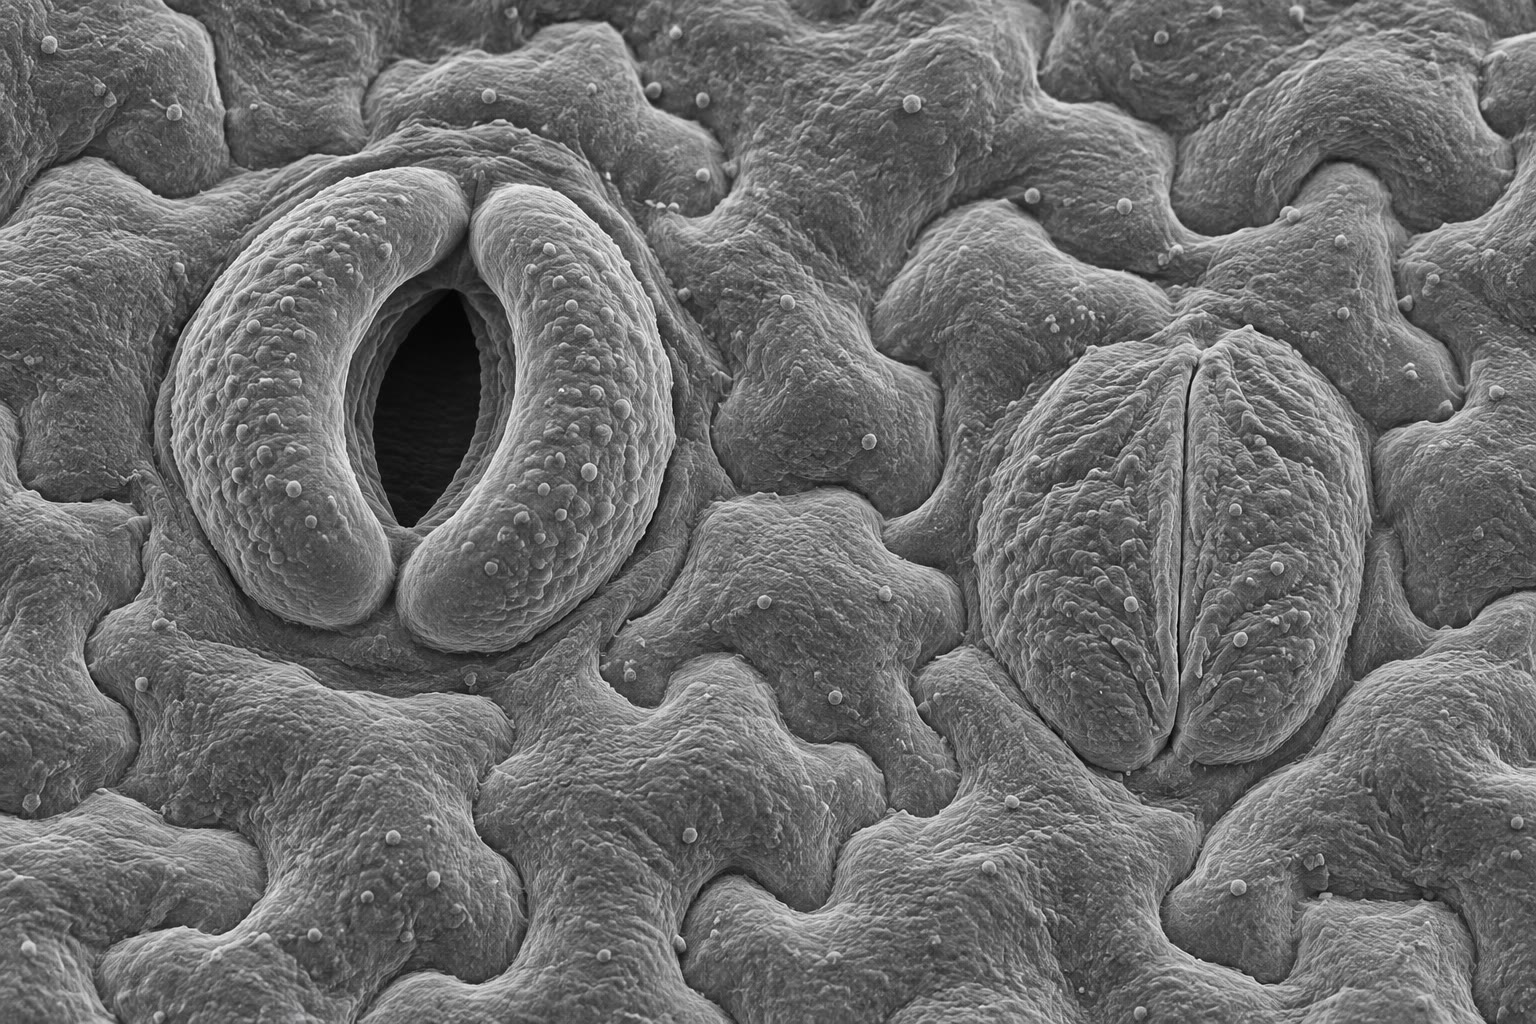
\includegraphics[width=0.46\linewidth]{images/book5/ai/b5-22-stomata-sem.jpg}\hspace{0.04\linewidth}
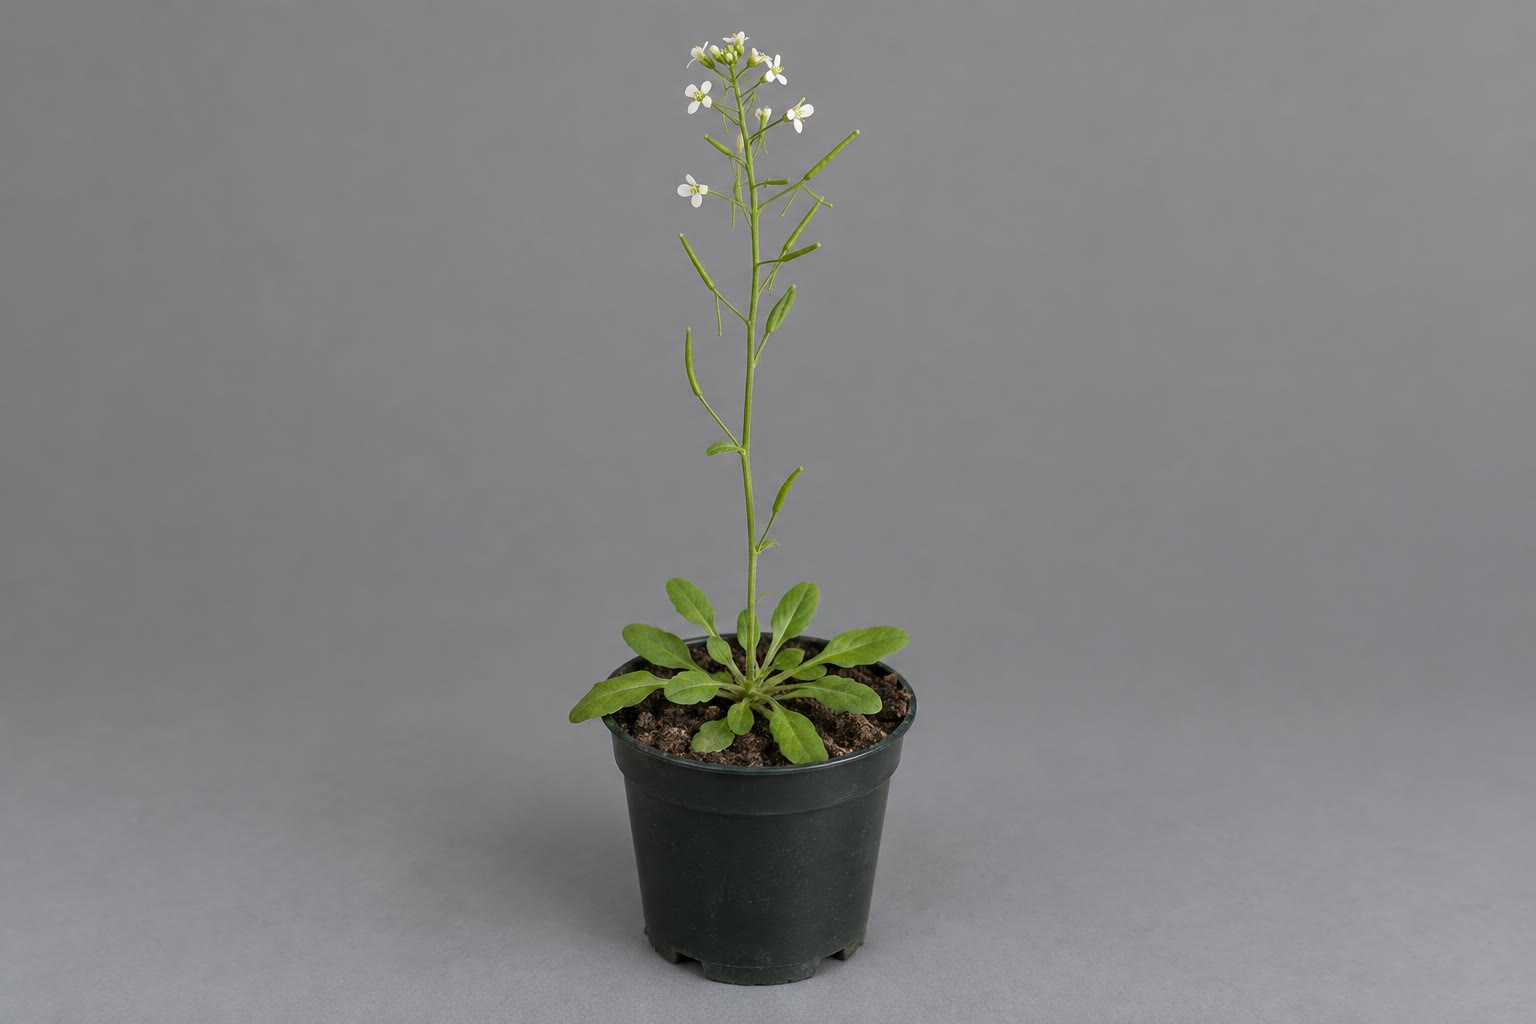
\includegraphics[width=0.46\linewidth]{images/book5/ai/b5-22-arabidopsis.jpg}

{\small Links: huidmondjes op een bladoppervlak, elke opening tussen
haar twee \omterm{prop:b3:plant-molecular-physiology:stomata}{sluitcellen}, sommige open en sommige dicht. Rechts:
\emph{Arabidopsis thaliana}, een bermonkruid met een klein genoom, een
generatie van zes weken en honderdduizend mutantenlijnen, waarin de
meeste moleculen van dit hoofdstuk zijn gevonden.}
\end{omfigure}

\section{Afweer zonder afweercellen}

\begin{definition}[Twee lagen van de plantenafweer]\label{def:b3:plant-molecular-physiology:immunity}
\index{door patronen opgewekte afweer}\index{door effectoren opgewekte afweer}\index{NLR-receptor}\index{overgevoeligheidsreactie}\index{systemisch verworven resistentie}\index{salicylzuur}\index{jasmonzuur}
Elke plantencel is haar eigen afweercel. De eerste laag, de \emph{door
patronen opgewekte afweer} (PTI), gebruikt receptorkinasen aan het
oppervlak die moleculen herkennen welke hele klassen microben gemeen
hebben --- FLS2 bindt een stuk bacterieel flagelline van 22 aminozuren,
andere binden chitinefragmenten van schimmelwanden --- en zet binnen
minuten een instroom van calcium, een uitbarsting van reactieve
zuurstof, kinasecascades, de sluiting van de huidmondjes, verdikking
van de wand met callose en de transcriptie van honderden afweergenen in
gang; zij houdt de meeste microben tegen. Ziekteverwekkers die toch
slagen spuiten \emph{effectoren} in --- eiwitten die onderdelen van de
PTI onklaar maken --- en daartegen zet de tweede laag, de \emph{door
effectoren opgewekte afweer} (ETI), intracellulaire
\emph{NLR-receptoren} in (nucleotidebindend, met leucinerijke
herhalingen), die elk één effector herkennen of de schade die hij
aanricht, in de paarsgewijze koppeling van gen tegen gen die Flor bij
de roest van vlas beschreef (jaren 1940). ETI is sneller en sterker dan
PTI en eindigt gewoonlijk in de \emph{overgevoeligheidsreactie}: de
besmette cel en haar buren doden zichzelf en muren de ziekteverwekker
in dood weefsel in --- de kleine bruine vlekjes op een resistent blad.
Beide lagen maken \omterm{def:b3:endocrinology:hormone}{hormonen} vrij die het alarm dragen:
\emph{salicylzuur} tegen biotrofen (die van levende cellen leven), wat
weken lang in de hele plant de \emph{systemisch verworven resistentie}
opwekt; \emph{jasmonzuur} en \omterm{def:b3:plant-molecular-physiology:hormones}{ethyleen} tegen necrotrofen (die eerst
doden en dan eten) en tegen knagende insecten, waarbij vluchtige
jasmonaten naburige planten waarschuwen en de sluipwespen van de
insecten aantrekken. De twee \omterm{def:b3:endocrinology:hormone}{hormonen} werken elkaar tegen, en sommige
ziekteverwekkers buiten dat uit: een bacterie die een nabootsing van
jasmonaat maakt zet de salicylaatafweer uit die haar zou hebben
gestopt.
\end{definition}

\begin{omfigure}
\begin{tikzpicture}
\begin{axis}[
  width=0.78\linewidth, height=5.4cm,
  axis x line=bottom, axis y line=left,
  xmin=0, xmax=10, ymin=0, ymax=10,
  xlabel={de wapenwedloop, van links naar rechts}, ylabel={sterkte van de afweer},
  xlabel style={font=\small, at={(axis description cs:0.5,-0.08)}, anchor=north}, ylabel style={font=\small},
  xtick=\empty, ytick=\empty,
  clip=false,
]
\addplot[very thick, omDef] coordinates {(0,1) (1.5,5)};
\addplot[very thick, omThm] coordinates {(1.5,5) (3.2,1.8)};
\addplot[very thick, omDef] coordinates {(3.2,1.8) (4.8,8)};
\addplot[very thick, omThm] coordinates {(4.8,8) (6.4,2.2)};
\addplot[very thick, omDef] coordinates {(6.4,2.2) (8.0,8.6)};
\draw[dashed, gray] (axis cs:0,4) -- (axis cs:8.5,4); \node[font=\scriptsize, gray, anchor=west] at (axis cs:8.5,4) {drempel van resistentie};
\draw[dashed, gray] (axis cs:0,7.2) -- (axis cs:8.5,7.2); \node[font=\scriptsize, gray, anchor=west] at (axis cs:8.5,7.2) {overgevoeligheidsreactie};
\node[font=\scriptsize, omDef, anchor=south west] at (axis cs:0.1,5.3) {PTI: receptoren zien flagelline, chitine};
\node[font=\scriptsize, omThm, anchor=north, align=center] at (axis cs:3.2,1.6) {effectoren ingespoten:\\PTI onklaar};
\node[font=\scriptsize, omDef, anchor=south, align=center] at (axis cs:4.8,8.2) {ETI: een NLR herkent\\een effector};
\node[font=\scriptsize, omThm, anchor=north, align=center] at (axis cs:6.4,2.0) {effector verloren of veranderd:\\herkenning ontlopen};
\node[font=\scriptsize, omDef, anchor=south, align=center] at (axis cs:8.0,8.8) {een nieuwe NLR\\ontstaat};
\end{axis}
\end{tikzpicture}

{\small De zigzag van de coëvolutie van plant en ziekteverwekker.
Receptoren aan het oppervlak wekken een afweer op tegen algemene
microbiële moleculen; ziekteverwekkers spuiten effectoren in die haar
onderdrukken; planten ontwikkelen intracellulaire receptoren voor de
effectoren; ziekteverwekkers laten ze vallen of veranderen ze; en zo
voort, waarbij elke stap genen voor resistentie en virulentie
achterlaat waarmee kwekers en ziekteverwekkers nog altijd handelen.}
\end{omfigure}

\begin{proof}[Bewijsmateriaal]
Flor (jaren 1940) kruiste vlasrassen en roeststammen en vond dat de
resistentie tegen elke stam uitsplitste als één dominant gen van de
plant, gepaard aan één avirulentiegen in de schimmel --- de
gen-tegen-genrelatie, vijftig jaar lang onverklaard tot de eerste
NLR-genen werden gekloneerd (1994) en de eerste paren van effector en
receptor bleken elkaar te binden of elkaars schade te merken.
Gómez-Gómez en Boller (2000) vonden de mutant van \emph{Arabidopsis}
die blind is voor flagelline, \emph{fls2}, en toonden dat haar
receptorkinase het peptide flg22 bij nanomolaire concentratie bond en
dat de mutant vatbaarder was voor bacteriën die op haar bladeren werden
gesproeid maar niet voor bacteriën die erin werden gespoten --- de
receptor bewaakt het oppervlak en de huidmondjes waardoor bacteriën
binnenkomen. Ross (1961) entte één blad van een tabaksplant met een
\omterm{def:b3:virology:virus}{virus} en vond de andere bladeren een week later resistent: de
\omterm{def:b3:plant-molecular-physiology:immunity}{systemisch verworven resistentie}, waarvan later bleek dat zij
\omterm{def:b3:plant-molecular-physiology:immunity}{salicylzuur} nodig heeft, dat de plant maakt langs dezelfde route als de
moederstof van aspirine.
\end{proof}

\begin{example}[De klok van de plant en de lengte van de dag]\label{ex:b3:plant-molecular-physiology:clock}
Planten houden een \omterm{def:b3:endocrinology:clock}{circadiane klok} van hetzelfde ontwerp als die van
het dier en uit niet-verwante onderdelen: ochtendfactoren (CCA1, LHY)
onderdrukken een avondgen (TOC1) wier product hen onderdrukt, met nog
meer lussen die zelfs bij aanhoudend licht een robuuste cyclus van 24
uur opleveren en de dageraad een uur van tevoren aankondigen door de
huidmondjes te openen en de genen van de fotosynthese aan te zetten. De
gevolgrijkste uitvoer van de klok is het meten van de daglengte. Bij
\emph{Arabidopsis}, een langedagplant, laat de klok het CONSTANS-eiwit
zich in de late middag ophopen; is die middag in een lange dag nog
belicht, dan stabiliseren \omterm{def:b3:plant-molecular-physiology:photoreceptors}{fytochroom} en \omterm{def:b3:plant-molecular-physiology:photoreceptors}{cryptochroom} het eiwit en zet
het \emph{FT} in het blad aan; in een korte dag wordt het eiwit in het
donker gemaakt en vernietigd. Het FT-eiwit, het florigeen waarop
entproeven sinds Chailakhyan (1936) jacht maakten, reist door het
floëem naar de scheuttop en zet die daar, met een partner, van het
maken van bladeren om naar het maken van bloemen. Kortedagplanten
(rijst, soja) gebruiken dezelfde klok met omgekeerd teken. Een plant
leest dus de kalender door een intern ritme met het externe licht te
vergelijken --- het ``uitwendige samenvallen'' dat Bünning in 1936
voorstelde en dat de moleculaire genetica zeventig jaar later
letterlijk maakte.
\end{example}

\begin{remark}[Stilstaan en alles veranderen]\label{rem:b3:plant-molecular-physiology:remark}
Het antwoord van het dier op een slechte omgeving is haar te verlaten;
dat van de plant is een andere plant te worden. Zij heeft receptoren
voor de kleur en de richting van het licht, de trek van de
zwaartekracht, de waterpotentiaal van haar bodem, de aanraking van de
wind en de chemie van haar vijanden; haar \omterm{def:b3:endocrinology:hormone}{hormonen} werken door
repressoren te vernietigen, zodat een signaal in minuten een programma
kan omschakelen; en elke cel is haar eigen voeler, haar eigen
afweersysteem en, als het moet, haar eigen regenererende meristeem. De
dwergtarwes die een groeiende wereld hebben gevoed waren een
DELLA-eiwit dat niet kon worden afgebroken; de droogtebestendige
gewassen van de komende decennia zullen voor een groot deel een kwestie
zijn van ABA-receptoren, de geleiding van de huidmondjes en de
watergebruiksefficiëntie die dit hoofdstuk heeft berekend.
\end{remark}

\section{Opgaven}

\begin{exercise}[$\star$]\label{exo:b3:plant-molecular-physiology:1}
Noem de drie families fotoreceptoren met hun golflengten en van elk één
reactie. Waarom heeft een plant fotoreceptoren nodig terwijl zij al
chlorofyl heeft?
\end{exercise}

\begin{exercise}[$\star$]\label{exo:b3:plant-molecular-physiology:2}
Leg uit hoe \omterm{def:b3:plant-molecular-physiology:hormones}{auxine}, \omterm{def:b3:plant-molecular-physiology:hormones}{gibberelline} en jasmonaat een werkingsmechanisme
delen, en waarom het antwoord daardoor snel is.
\end{exercise}

\begin{exercise}[$\star$]\label{exo:b3:plant-molecular-physiology:3}
Beschrijf de opeenvolging van gebeurtenissen vanaf de aankomst van ABA
bij een \omterm{prop:b3:plant-molecular-physiology:stomata}{sluitcel} tot het sluiten van de opening, en noem het punt waar
een mutatie de plant haar huidmondjes niet meer zou laten sluiten.
\end{exercise}

\begin{exercise}[$\star$]\label{exo:b3:plant-molecular-physiology:4}
Onderscheid de door patronen opgewekte en de \omterm{def:b3:plant-molecular-physiology:immunity}{door effectoren opgewekte
afweer} naar wat er wordt herkend, waar de receptor zit, en hoe het
antwoord eindigt.
\end{exercise}

\begin{exercise}[$\star\star$]\label{exo:b3:plant-molecular-physiology:5}
Bereken met de fit $\varphi \approx 0.87\,\zeta/(\zeta + 0.6)$ het
Pfr-deel in daglicht ($\zeta = 1.15$), onder één blad ($\zeta =
0.4$), onder een dicht bladerdak ($\zeta = 0.1$) en onder een gloeilamp
($\zeta = 0.7$). Waarom worden kiemplanten onder zulke lampen lang?
\end{exercise}

\begin{exercise}[$\star\star$]\label{exo:b3:plant-molecular-physiology:6}
Bereken de verhouding binnen:buiten voor \omterm{def:b3:plant-molecular-physiology:hormones}{auxine} als de pH van de
celwand $5.0$ is en die van het cytosol $7.5$; en daarna als de wand
tot $4.5$ wordt aangezuurd (zoals groeiende cellen doen). Wat gebeurt
er met de val als het cytosol bij zuurstofgebrek tot $6.5$ aanzuurt?
\end{exercise}

\begin{exercise}[$\star\star$]\label{exo:b3:plant-molecular-physiology:7}
\omterm{def:b3:plant-molecular-physiology:hormones}{Auxine} beweegt met \qty{1}{cm/h} door cellen van \qty{50}{\micro m}
lang. Hoeveel cellen doorkruist het per uur, en hoe lang blijft het in
elke cel? Vergelijk met de tijd om \qty{50}{\micro m} te diffunderen ($D =
\qty{5e-10}{m^2/s}$, $t \approx x^{2}/2D$) en zeg welke stap het
transport begrenst.
\end{exercise}

\begin{exercise}[$\star\star$]\label{exo:b3:plant-molecular-physiology:8}
Een blad bij \qty{25}{\celsius} heeft binnen een molfractie waterdamp
van \qty{32}{mmol/mol} en de lucht \qty{16}{mmol/mol}; CO$_{2}$ is
\qty{400}{ppm} buiten en \qty{250}{ppm} binnen. Bereken het aantal
watermoleculen dat per vastgelegd CO$_{2}$ verloren gaat. Bereken
opnieuw voor een C$_{4}$-plant met intern CO$_{2}$ op \qty{150}{ppm},
en voor een droge dag met lucht op \qty{8}{mmol/mol}.
\end{exercise}

\begin{exercise}[$\star\star$]\label{exo:b3:plant-molecular-physiology:9}
Leg uit waarom een plant die aan koude is gewend vaak ook beter tegen
droogte kan, en noem de gedeelde signalen en beschermende moleculen.
\end{exercise}

\begin{exercise}[$\star\star\star$]\label{exo:b3:plant-molecular-physiology:10}
\omterm{def:b3:plant-molecular-physiology:photoreceptors}{Fytochroom} nadert zijn \omterm{prop:b3:plant-molecular-physiology:photoequilibrium}{foto-evenwicht} met een snelheid $k_{1} + k_{2}$
die evenredig is met de stroom. Als volle zon $k_{1} + k_{2} =
\qty{0.5}{s^{-1}}$ geeft, hoe lang duurt de omschakeling dan bij de
\qty{1}{\%} van de volle zon in de dageraad? Pfr keert in het donker
terug met een halveringstijd van \qty{2}{h}: welk deel blijft er over
na een nacht van acht uur, en hoe laat dit een zaad een korte
blootstelling van een dag onderscheiden?
\end{exercise}

\begin{exercise}[$\star\star\star$]\label{exo:b3:plant-molecular-physiology:11}
De \omterm{def:b3:plant-molecular-physiology:immunity}{overgevoeligheidsreactie} doodt per besmettingsplek misschien honderd
cellen. Beredeneer met een ruwe kosten-batenschatting voor een blad van
$10^{7}$ cellen dat per dag tien besmettingen te verduren krijgt,
waarom zelfmoord van besmette cellen goedkoop is, en waarom een
necrotroof (die van dode cellen leeft) deze afweer in een zwakte
verandert.
\end{exercise}

\begin{exercise}[$\star\star\star$]\label{exo:b3:plant-molecular-physiology:12}
Modelleer het uitwendige samenvallen: het CONSTANS-eiwit wordt tussen
uur 12 en uur 16 na de dageraad gemaakt en met een halveringstijd van
\qty{30}{min} in het donker maar \qty{4}{h} in het licht afgebroken.
Schat het eiwit dat er op uur 16 over is bij een dag van 16 uur en bij
een dag van 10 uur (donker vanaf uur 10), en leg uit hoe een drempel
dit in een besluit tot bloeien omzet.
\end{exercise}

\section{Vraagstuk: een kiemplant in de schaduw}

\begin{problem}[{Weekendvraagstuk --- een kiemplant gelezen door haar
moleculen: de fytochroombalans onder een bladerdak, het auxine dat zij
vangt en vervoert, het water dat zij via haar huidmondjes tegen
koolstof ruilt, en de kosten van het verdedigen van haar bladeren,
eindigend bij het Pfr-deel onder het bladerdak, de valverhouding van
het auxine en de watergebruiksefficiëntie}]
\label{pb:b3:plant-molecular-physiology:1}
Gegevens: fit van het \omterm{prop:b3:plant-molecular-physiology:photoequilibrium}{foto-evenwicht} $\varphi = 0.87\,\zeta/(\zeta + 0.6)$;
daglicht $\zeta = 1.15$, bladerdak $\zeta = 0.2$; strekkingssnelheid
van het hypocotyl $r = r_{0}(1 - \varphi)$ met $r_{0} = \qty{2}{mm/h}$.
\omterm{def:b3:plant-molecular-physiology:hormones}{Auxine} $\mathrm{p}K_{a} = 4.75$; pH van de celwand $5.5$, van het
cytosol $7.2$; transportsnelheid \qty{1}{cm/h}; cellengte
\qty{100}{\micro m}. Blad: molfractie waterdamp binnen
\qty{32}{mmol/mol}, lucht \qty{16}{mmol/mol}; CO$_{2}$ \qty{400}{ppm}
buiten, \qty{250}{ppm} binnen; $g_{s} =
\qty{0.3}{mol\,m^{-2}\,s^{-1}}$ (waterdamp); bladoppervlak
\qty{20}{cm^2}; \qty{12}{h} licht. Afweer: de \omterm{def:b3:plant-molecular-physiology:immunity}{overgevoeligheidsreactie}
doodt $100$ cellen per plek; het blad heeft $10^{7}$ cellen; PTI kost
\qty{5}{\%} van de fotosynthese zolang zij actief is.

\medskip
\noindent\textbf{Deel I --- Licht.}
\begin{enumerate}
  \item Bereken $\varphi$ in daglicht en onder het bladerdak.
  \item De strekkingssnelheden in beide, en de extra lengte na
        \qty{48}{h} in de schaduw.
  \item Een blad van een buur haalt \qty{90}{\%} van het rood en
        \qty{20}{\%} van het verrood uit het daglicht weg. Bereken de
        nieuwe $\zeta$ en $\varphi$. Volstaat één blad om
        \omterm{prop:b3:plant-molecular-physiology:photoequilibrium}{schaduwontwijking} uit te lokken?
  \item Leg uit waarom $\varphi$ onafhankelijk is van de helderheid, en
        wat dat betekent voor een kiemplant op een bewolkte dag buiten.
  \item Volle zon geeft $k_{1} + k_{2} = \qty{0.5}{s^{-1}}$. Hoe lang
        duurt het om \qty{95}{\%} van het \omterm{prop:b3:plant-molecular-physiology:photoequilibrium}{foto-evenwicht} te bereiken in
        volle zon en bij \qty{1}{\%} daarvan?
  \item Het Pfr dat overdag is gemaakt keert terug met een
        halveringstijd van \qty{2}{h}. Welk deel blijft er over na
        \qty{8}{h} en na \qty{14}{h} donker; hoe zou een plant dit als
        nachtlengteklok kunnen gebruiken, en waarom is het een slechte?
\end{enumerate}

\medskip
\noindent\textbf{Deel II --- \omterm{def:b3:plant-molecular-physiology:hormones}{Auxine}.}
\begin{enumerate}[resume]
  \item Het deel van het \omterm{def:b3:plant-molecular-physiology:hormones}{auxine} dat neutraal IAAH is in de celwand en
        in het cytosol.
  \item Verhouding binnen:buiten bij evenwicht van IAAH. Als de celwand
        \qty{0.1}{\micro M} \omterm{def:b3:plant-molecular-physiology:hormones}{auxine} in totaal bevat, wat is dan de
        concentratie in het cytosol?
  \item Cellen die per uur worden doorkruist, en de verblijftijd per cel.
  \item Een scheut van \qty{5}{cm} lang: hoe lang duurt het voordat een
        verandering van het \omterm{def:b3:plant-molecular-physiology:hormones}{auxine} aan de top de basis bereikt?
        Vergelijk met het uur dat een scheut nodig heeft om naar het
        licht te beginnen buigen, en geef commentaar.
  \item In een zwaartekrachtgeprikkelde wortel verhuist PIN3 zo dat de
        onderste flank \qty{60}{\%} van de stroom ontvangt en de
        bovenste \qty{40}{\%}. Als de strekking van wortelcellen met
        \qty{1}{\%} daalt voor elke \qty{1}{\%} \omterm{def:b3:plant-molecular-physiology:hormones}{auxine} boven de norm en
        met evenveel stijgt eronder, bereken dan de snelheden van beide
        flanken ten opzichte van de norm, en de richting van de
        kromming.
  \item Waarom buigt dezelfde asymmetrie een scheut de andere kant op?
\end{enumerate}

\medskip
\noindent\textbf{Deel III --- Water voor koolstof.}
\begin{enumerate}[resume]
  \item Verdamping $E = g_{s}\,\Delta w$ in \unit{mmol\,m^{-2}\,s^{-1}}.
  \item Assimilatie $A = (g_{s}/1.6)\,\Delta c$ in \unit{\micro
        mol\,m^{-2}\,s^{-1}}, en de verhouding $E/A$.
  \item Water dat het blad van \qty{20}{cm^2} tijdens de dag van twaalf
        uur verliest, in mol en in gram; vastgelegde koolstof, in mol
        CO$_{2}$ en in gram glucose.
  \item ABA sluit de huidmondjes tot $g_{s} = \qty{0.05}{}$. Nieuwe $E$
        en $A$, en de verhouding. Wat heeft de plant gewonnen en verloren?
  \item Een C$_{4}$-plant houdt het interne CO$_{2}$ op \qty{150}{ppm}
        bij dezelfde $g_{s}$: haar $E/A$? Een CAM-plant opent 's nachts,
        wanneer $\Delta w = \qty{5}{mmol/mol}$: haar $E/A$ bij $\Delta c =
        \qty{150}{ppm}$?
  \item Leg uit waarom de verhouding $E/A$ niet van $g_{s}$ afhangt, en
        wat een plant eraan kan en niet kan doen.
\end{enumerate}

\medskip
\noindent\textbf{Deel IV --- Afweer.}
\begin{enumerate}[resume]
  \item Tien besmettingsplekken per dag, elk beantwoord met een
        \omterm{def:b3:plant-molecular-physiology:immunity}{overgevoeligheidsreactie}: gedode cellen per dag, als fractie
        van het blad.
  \item Welk deel wordt er in een bladleven van 60 dagen opgeofferd?
        Vergelijk met het verlies als één op de tien besmettingen
        ontsnapte en telkens \qty{5}{\%} van het blad vernietigde.
  \item PTI is \qty{20}{\%} van de tijd actief: de gemiddelde kosten
        als fractie van de fotosynthese. Waarom houden planten haar
        niet altijd aan?
  \item Een ziekteverwekker verwijdert de effector die een NLR herkent.
        Wat wint hij, wat verliest hij, en wat doet de plantenpopulatie
        daarna?
  \item Een bacterie scheidt een nabootsing van jasmonaat uit. Welke
        afweer zet zij daarmee uit, en waarom helpt haar dat, gegeven
        het antagonisme tussen de twee hormoonroutes?
  \item Waarom wordt een gen-tegen-genresistentie in een monocultuur
        vaak binnen een paar seizoenen verslagen, en wat stelt de
        zigzag voor dat kwekers in plaats daarvan doen?
  \item Vat samen: $\varphi$ onder het bladerdak (vraag~1), de
        valverhouding van het \omterm{def:b3:plant-molecular-physiology:hormones}{auxine} (vraag~8) en het aantal
        watermoleculen dat per vastgelegd CO$_{2}$ verloren gaat
        (vraag~14).
\end{enumerate}
\end{problem}
